\renewcommand{\thefigure}{B.\arabic{figure}}
\setcounter{figure}{0}

\section*{Appendix B: Calibration Logs and Supplementary Graphs}

Additional experimental relationships and fitting diagnostics are presented to support the main analysis.

\begin{figure}[H]
	\centering
	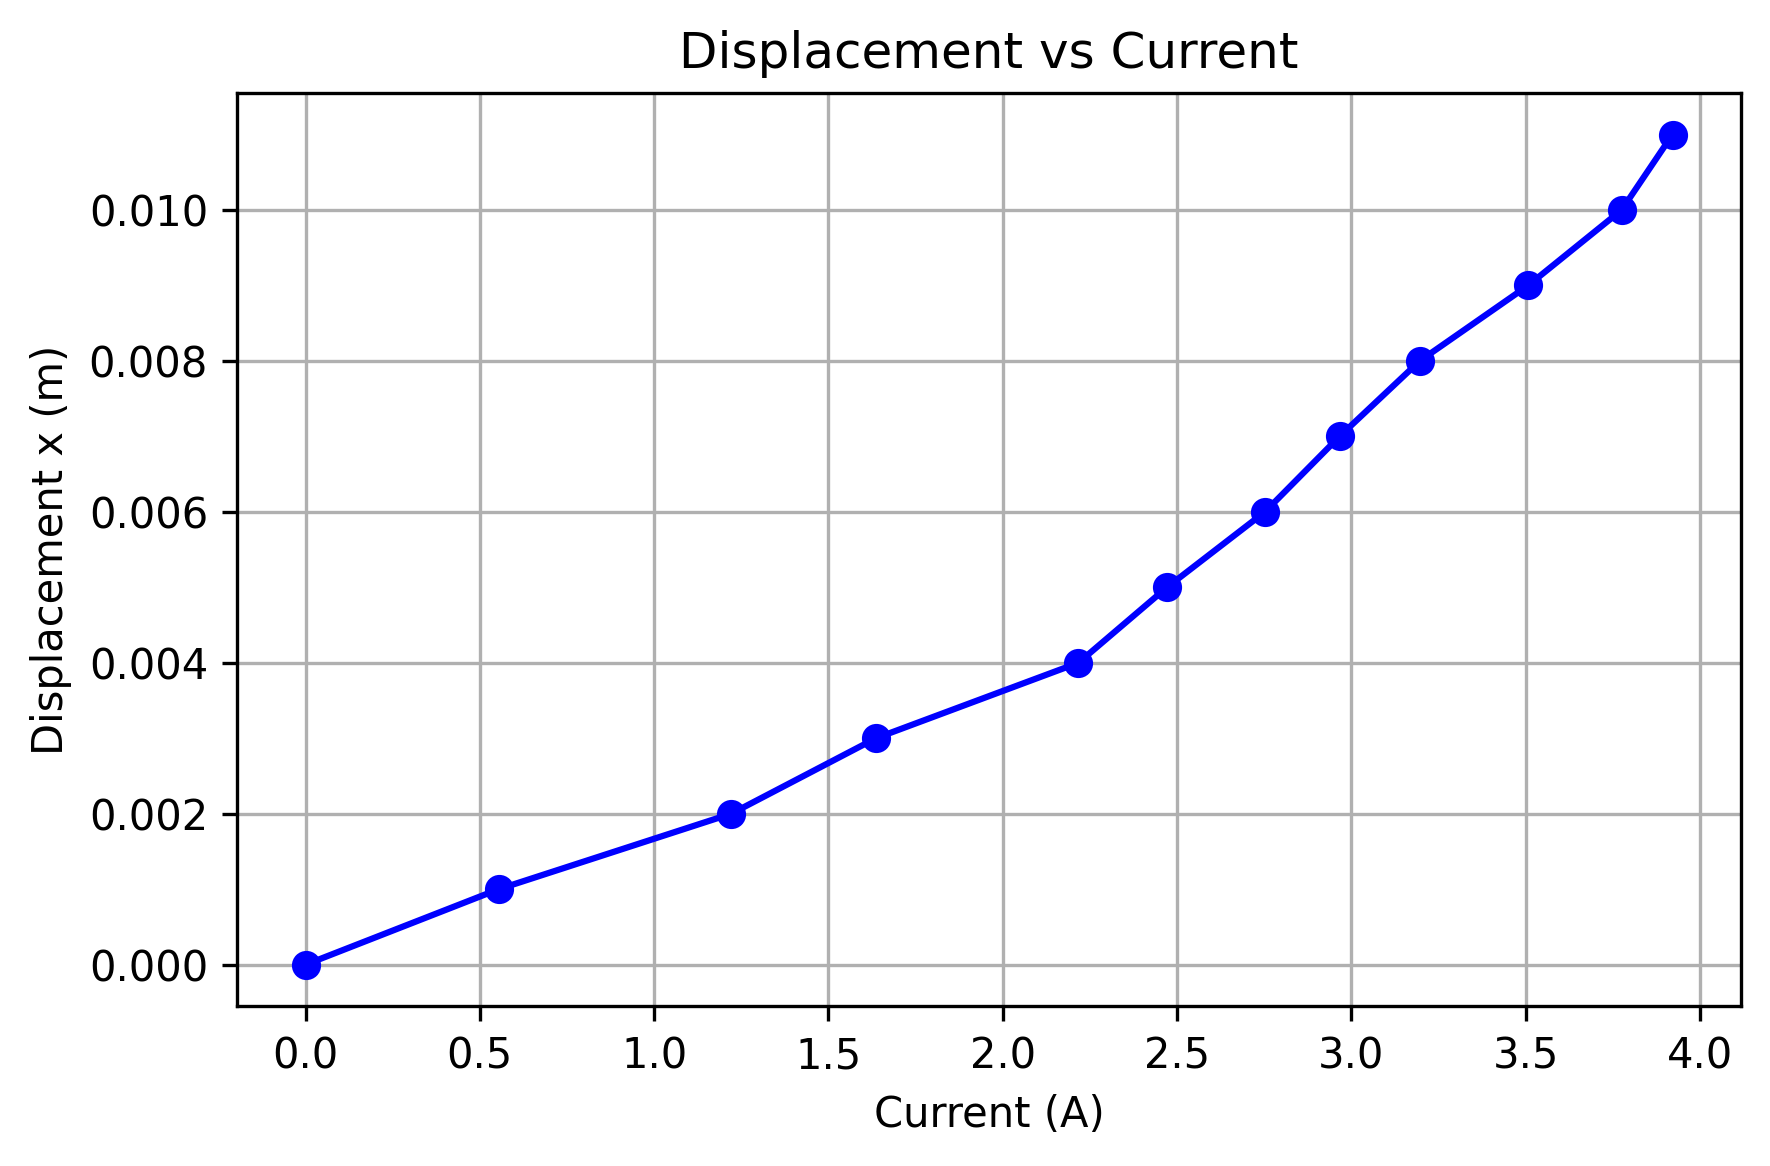
\includegraphics[width=0.85\textwidth]{Assests/Displacement_vs_Current.png}
	\caption{Displacement as a function of current through the solenoid.}
\end{figure}

\begin{figure}[H]
	\centering
	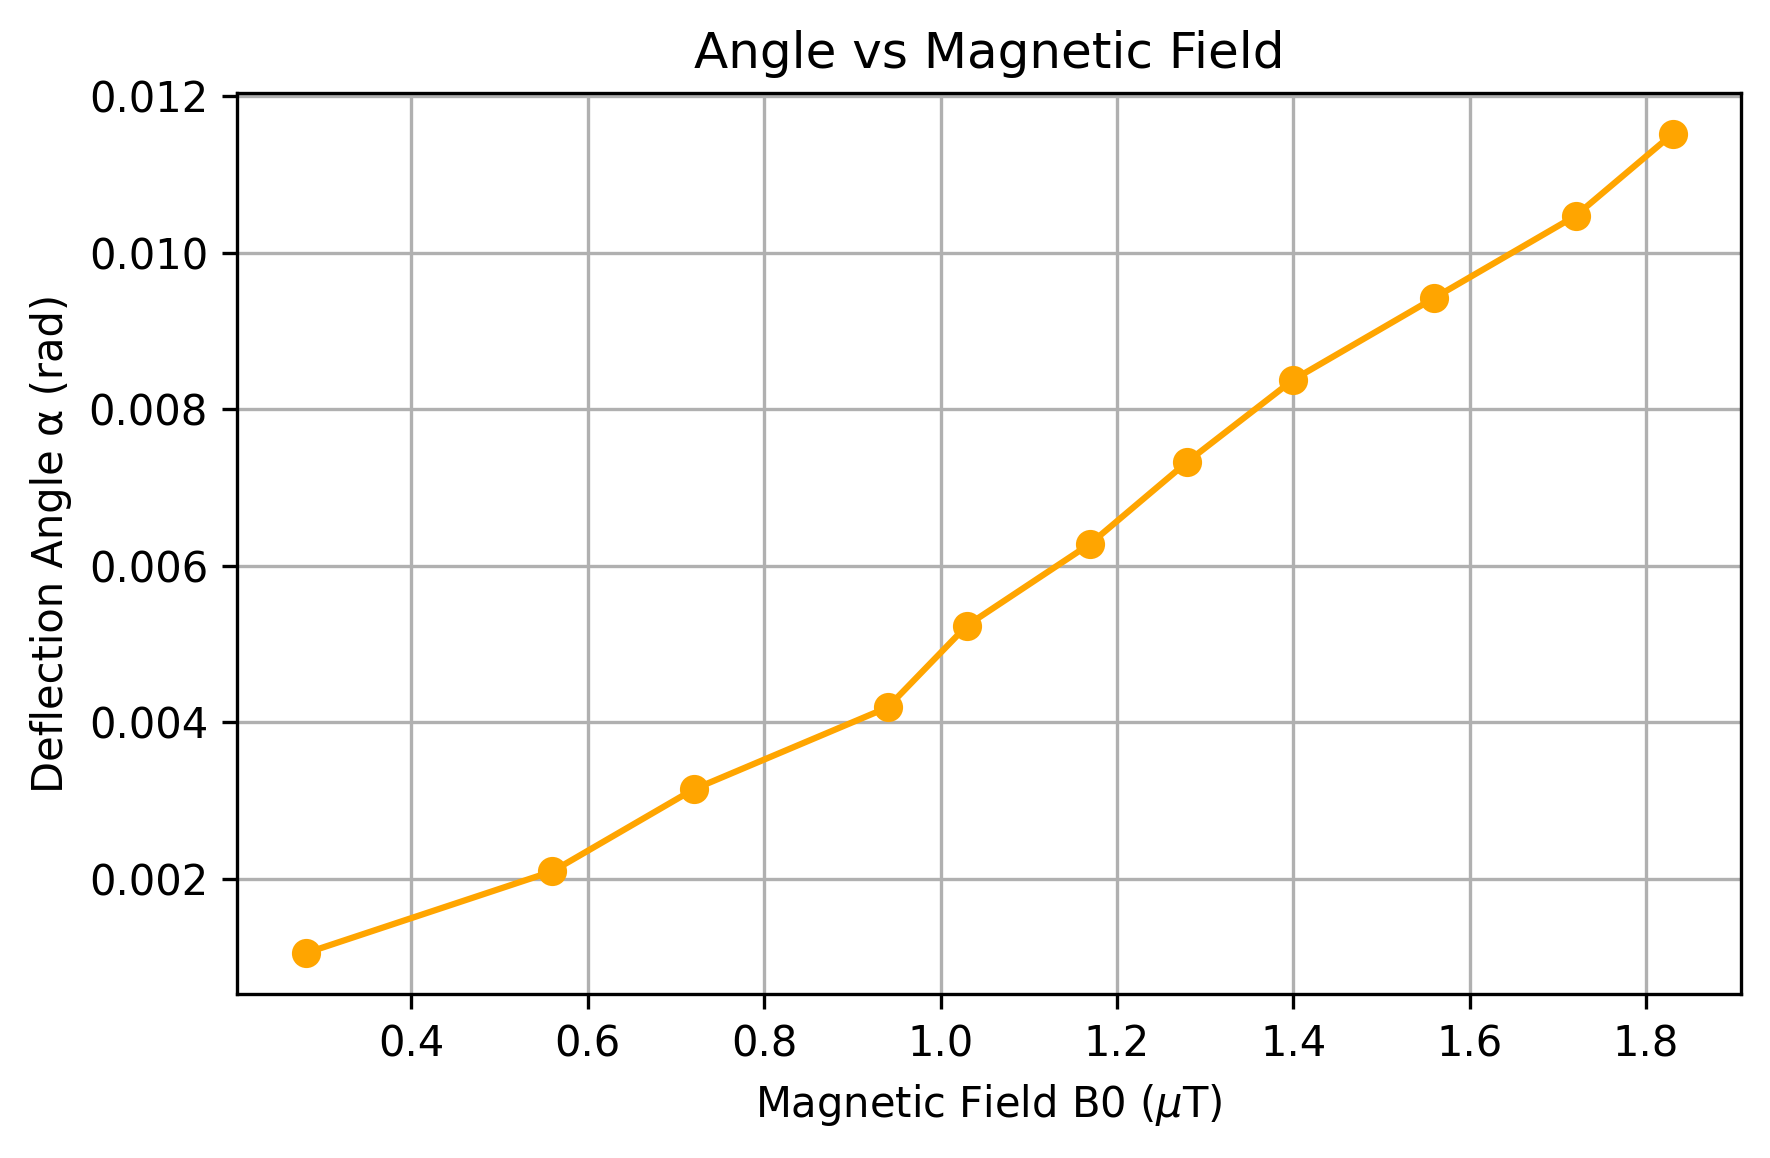
\includegraphics[width=0.85\textwidth]{Assests/Angle_vs_Field.png}
	\caption{Measured angle $\alpha$ versus magnetic field intensity $B_0$.}
\end{figure}

\begin{figure}[H]
	\centering
	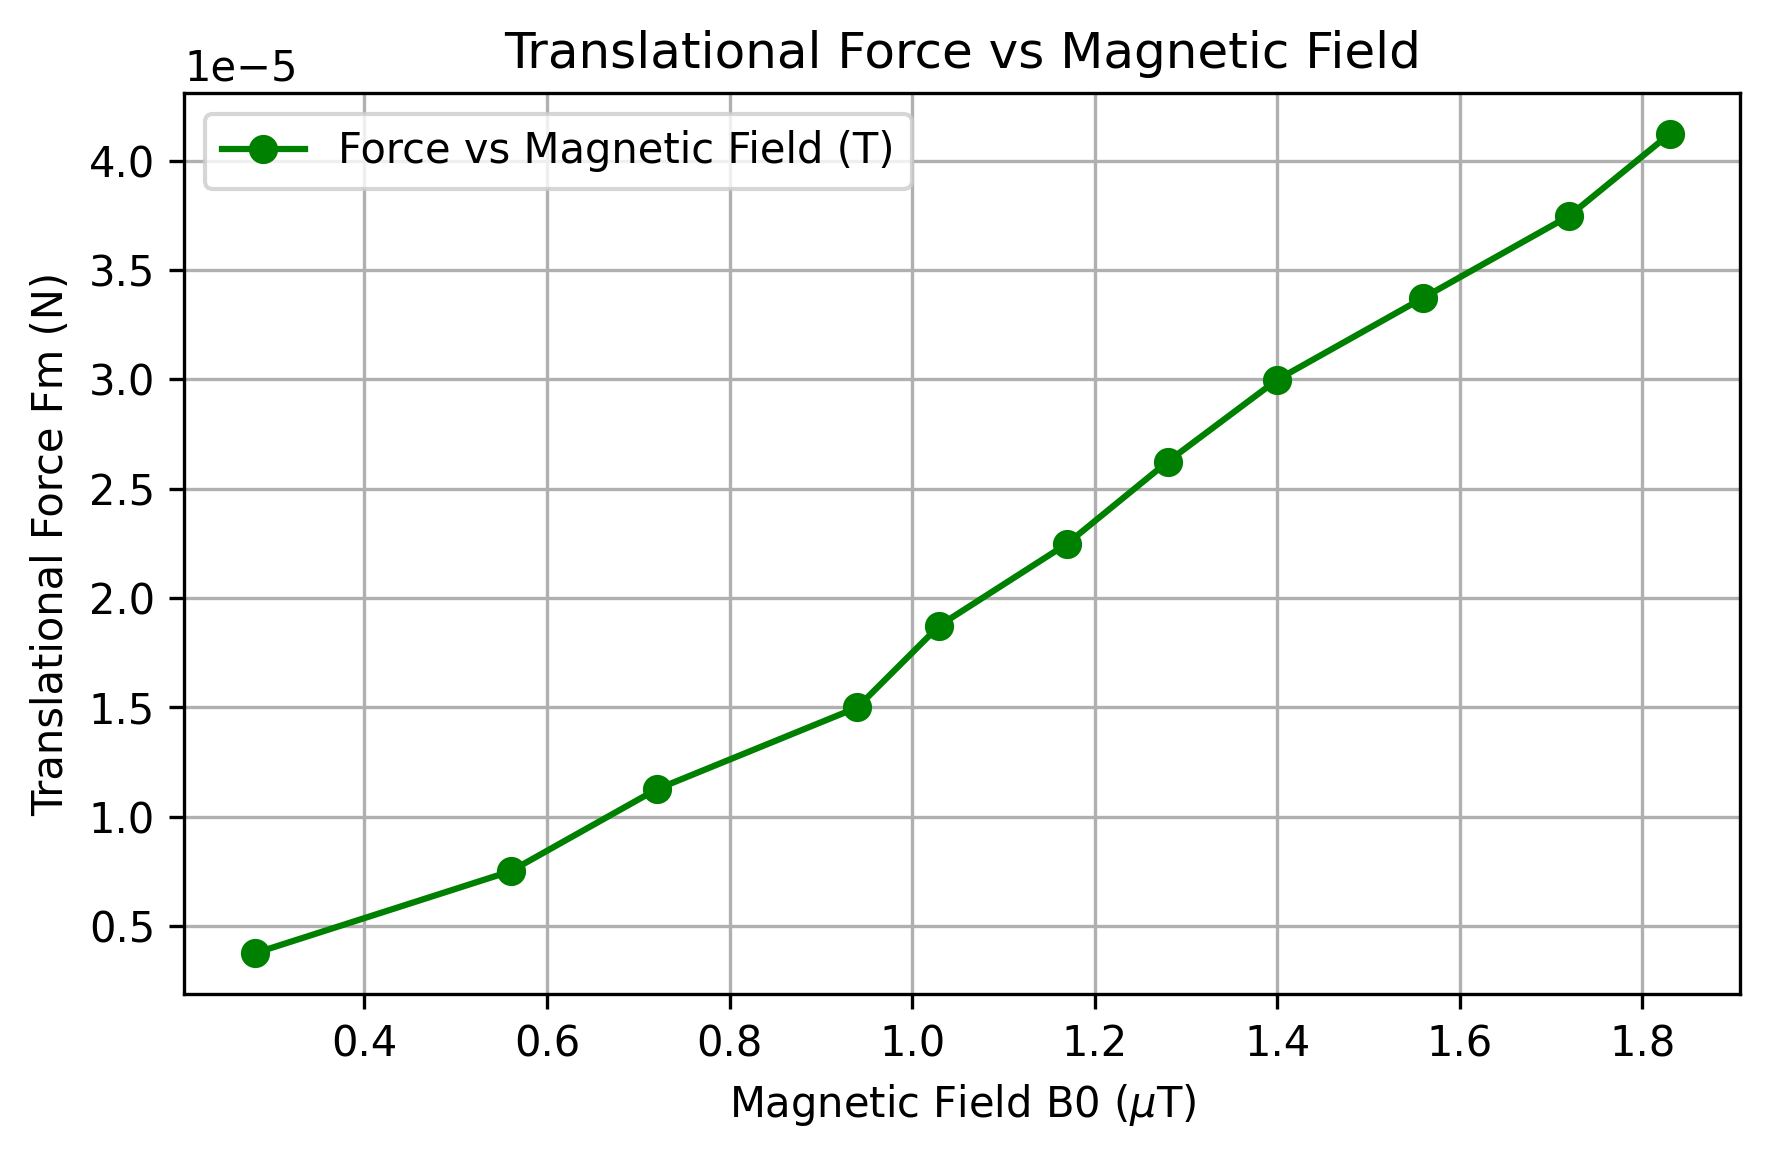
\includegraphics[width=0.85\textwidth]{Assests/Force_vs_Field.png}
	\caption{Computed translational force $F_m$ as a function of $B_0$.}
\end{figure}

\begin{figure}[H]
	\centering
	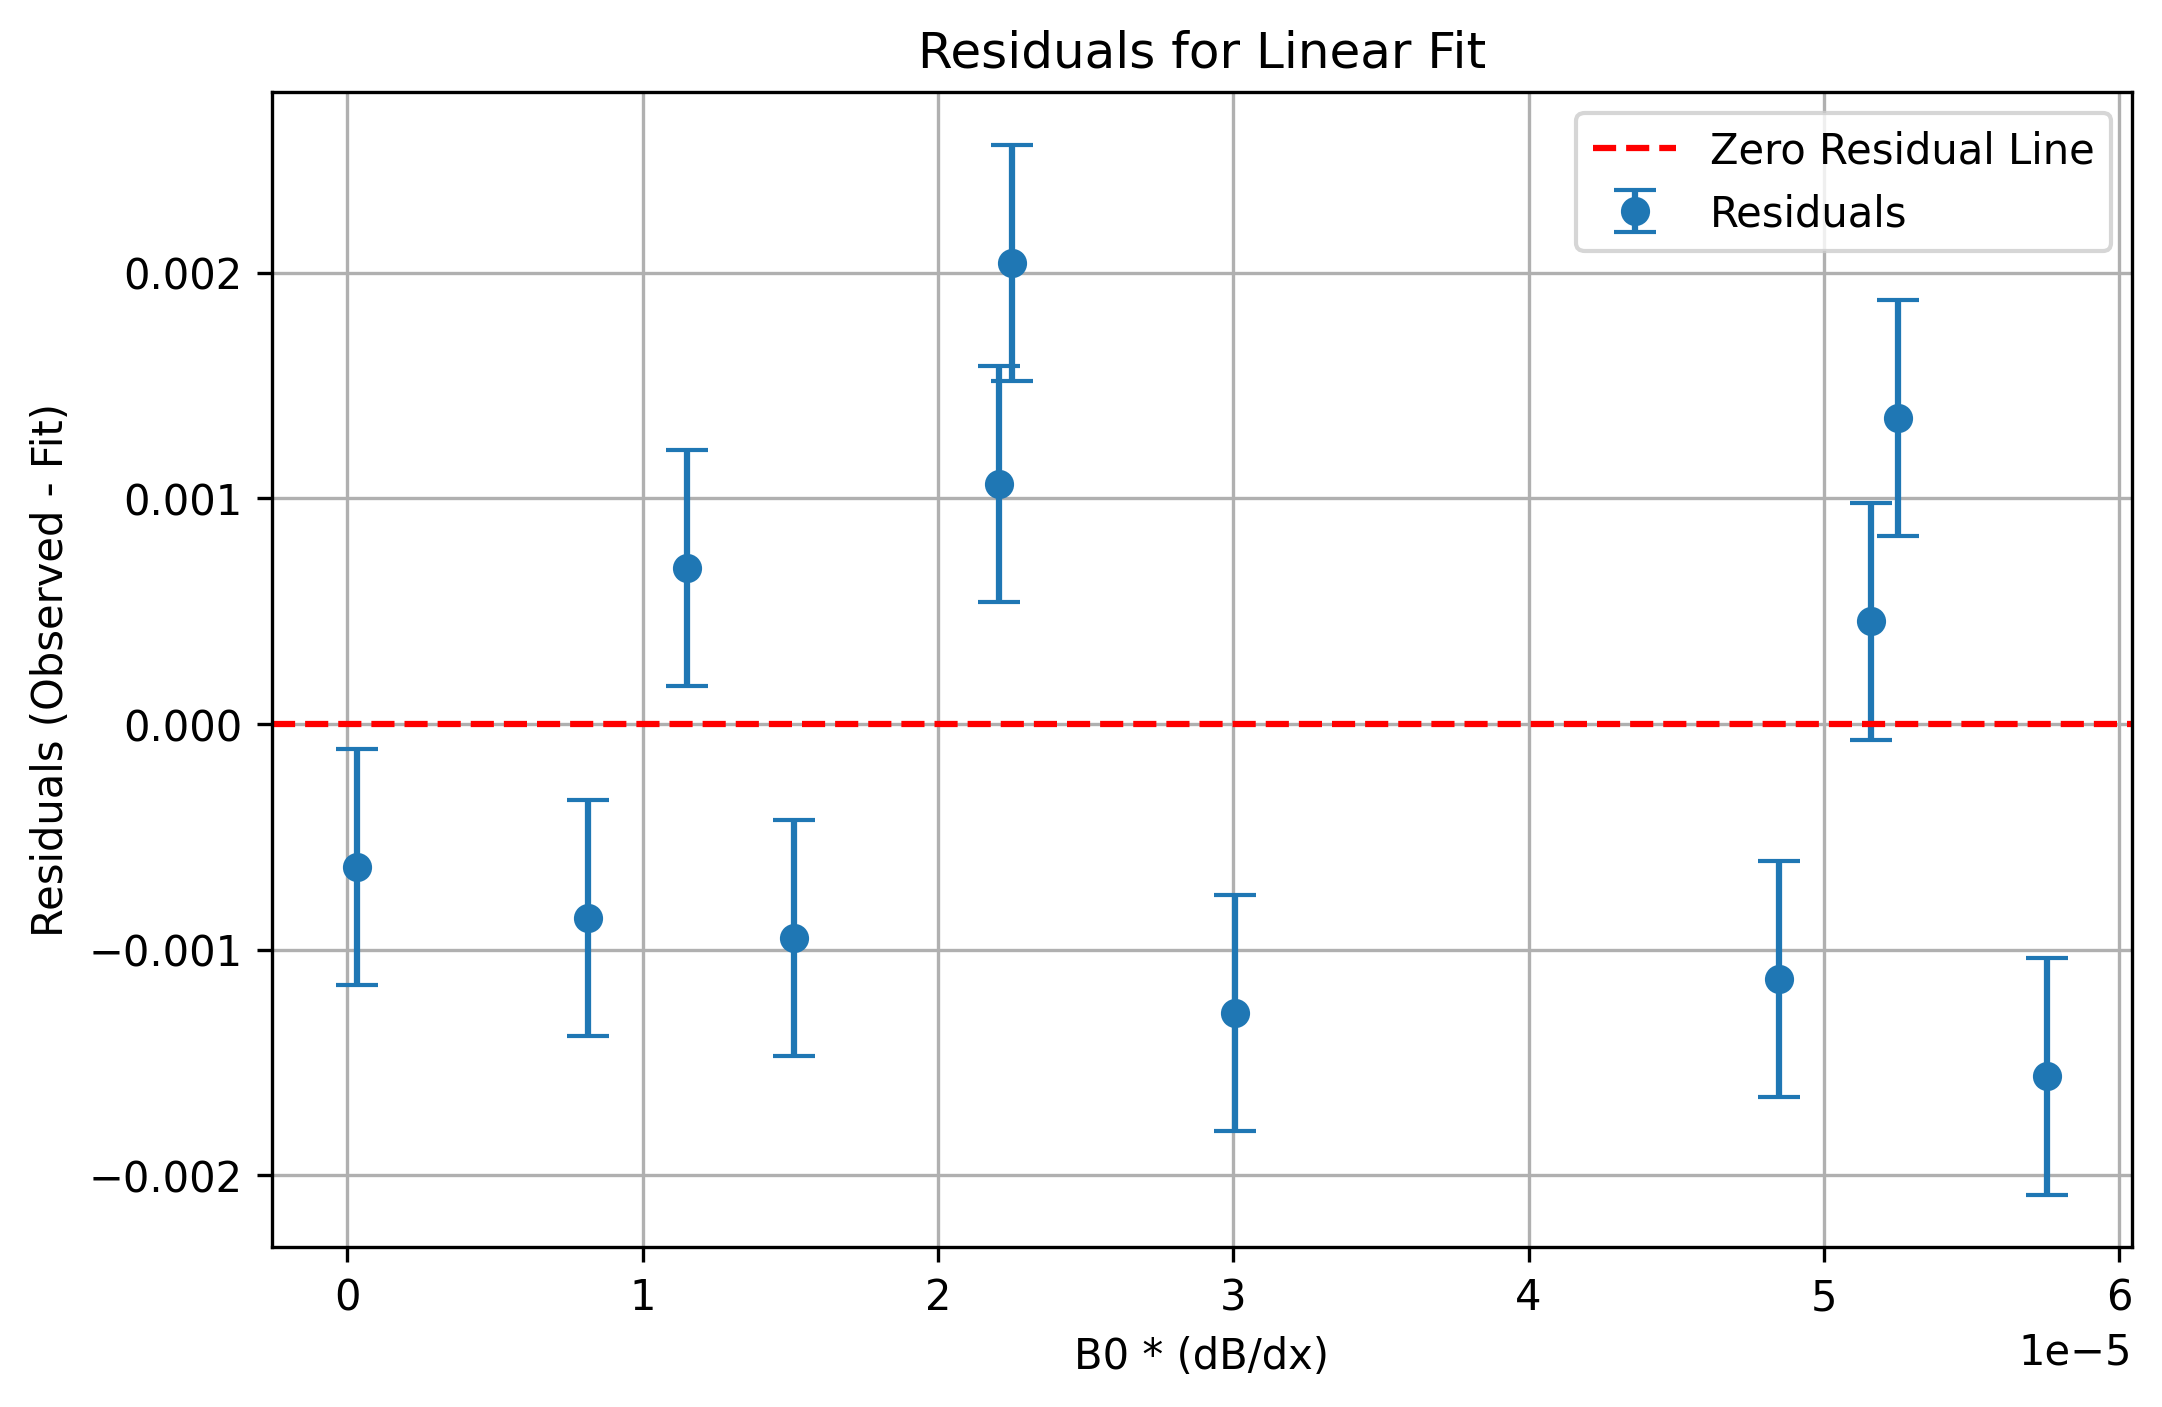
\includegraphics[width=0.85\textwidth]{Assests/Residuals_Plot.png}
	\caption{Residuals from linear fit of $\tan(\alpha)$ vs. $B_0 \cdot \frac{dB_0}{dz}$. Error bars indicate propagated uncertainties.}
\end{figure}

\begin{figure}[H]
	\centering
	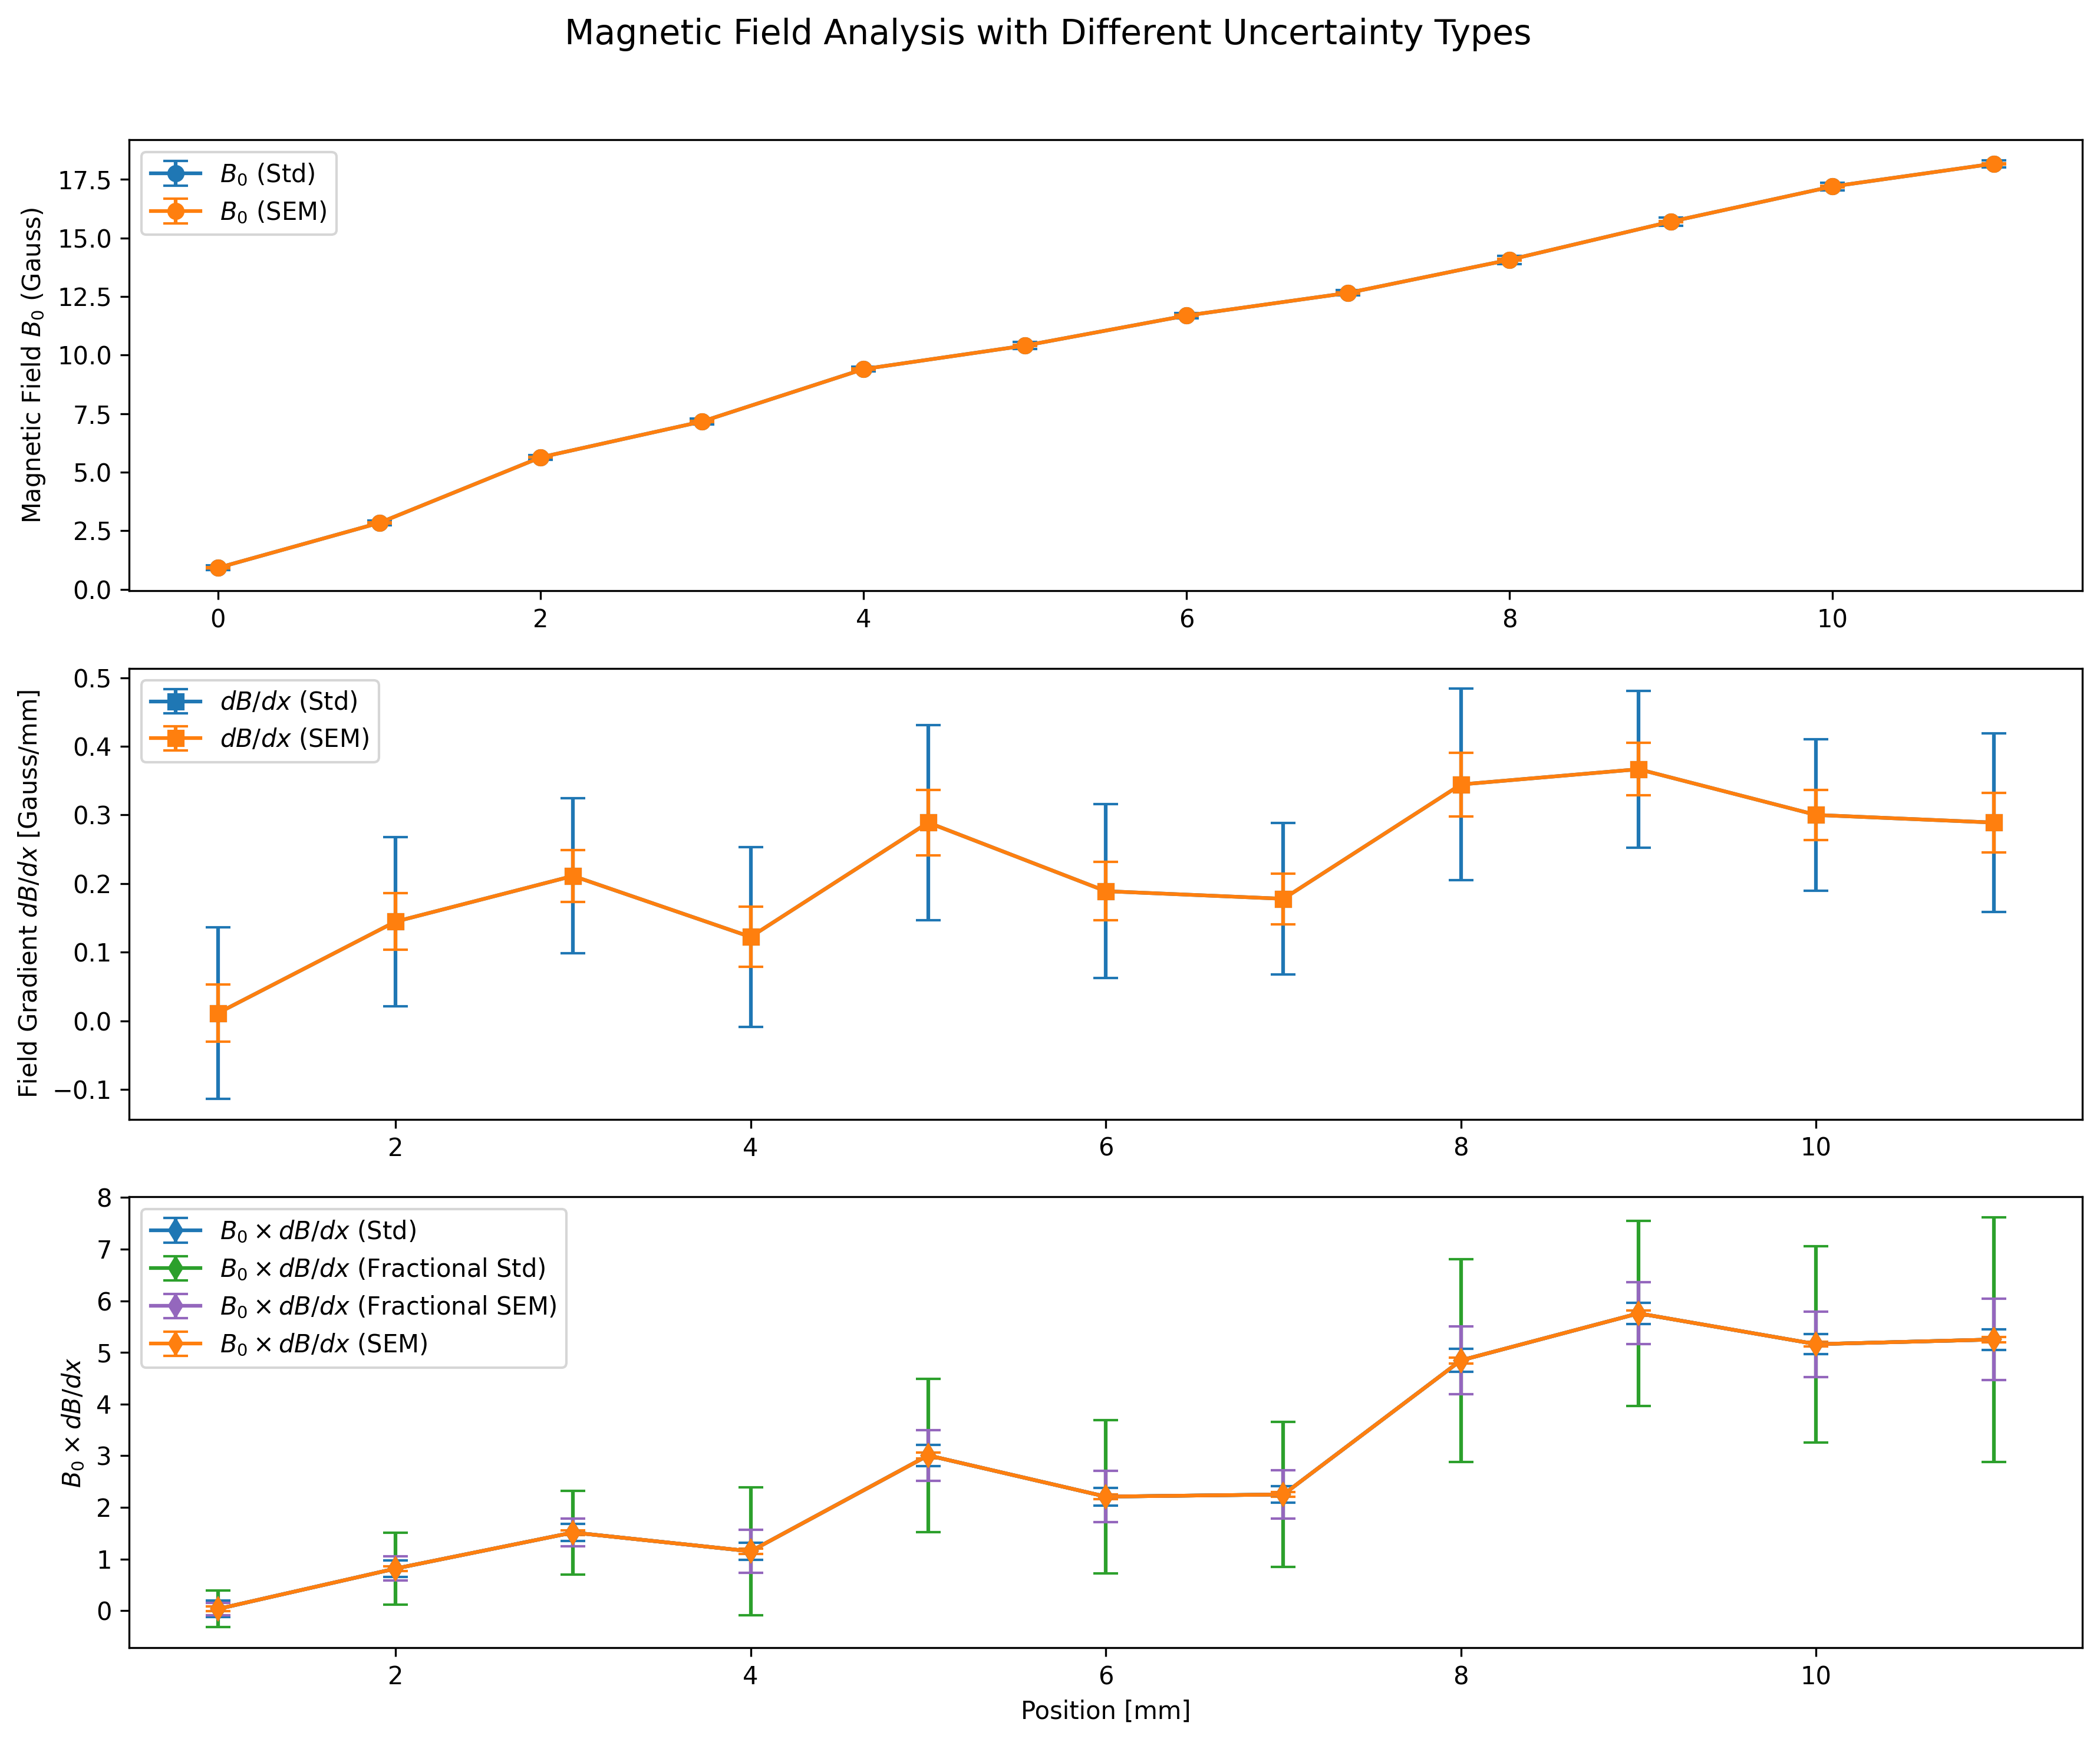
\includegraphics[width=\textwidth]{Assests/Uncertainty_Propagation_Plot.png}
	\caption{Propagation of measurement uncertainty through magnetic field analysis. Top: Measured field $B_0$ with standard deviation and SEM. Middle: Gradient $dB/dz$ with propagated error. Bottom: Final product $B_0 \cdot dB/dz$ with multiple uncertainty estimations (standard, fractional, SEM). This term was used as the independent variable in the susceptibility fit.}
	\label{fig:uncertainty}
\end{figure}